\documentclass{article}
\usepackage{graphicx}
\usepackage{amsmath}
\usepackage{amsfonts}
\usepackage{float}
\usepackage{hyperref}
\usepackage{listings}
\usepackage{color}
\usepackage{geometry}
\usepackage{subcaption}
\geometry{a4paper, margin=1in}

\title{Program 3a}
\author{Kevin Smith}
\date{\today}

\begin{document}

\maketitle

\section{Introduction}
The linear least squares method is a cornerstone in numerical analysis for solving overdetermined systems. This study extends to the regularized variant, which is pivotal in scenarios with noisy data. By implementing Householder reflectors and an incremental updating algorithm, we aim to provide efficient and accurate solutions to these problems.

\section{Problem Statement}
We consider the problem $\min_{x \in \mathbb{R}^k} \|b - Ax\|^2$, given $b \in \mathbb{R}^n$ and a matrix $A \in \mathbb{R}^{n \times k}$ with linearly independent columns. Additionally, we address the regularized version to improve the robustness against noise in the observations.

\section{Methodology}
\subsection{Implementation Details}
The algorithms are implemented in Python, utilizing numpy for matrix operations. The Householder-based approach transforms the problem into an upper triangular form, while the incremental algorithm updates the solution as new data arrives, suitable for real-time applications.

\subsection{Test Design}
The testing framework includes scenarios with known solutions, varying dimensions, and statistical behavior characterization. We ensure that the incremental code yields results consistent with the full-problem code.

\section{Results}
\subsection{Accuracy and Statistical Behavior}
Our tests confirm the accuracy of the implementations against known solutions. The incremental algorithm aligns with the full-problem algorithm, as shown by negligible discrepancies across a range of matrix sizes.

\subsection{Regularized Linear Least Squares}
The following figures illustrate signal reconstructions for various values of $n$ and regularization parameter $\lambda$. The reconstructions exhibit how an appropriate choice of $\lambda$ can significantly enhance the signal's fidelity, especially in the presence of noise.

\begin{figure*}[t!]
    \centering
    \caption{Signal reconstructions and error analysis for different problem sizes.}
    \label{fig:signal_reconstructions_and_error_analysis}
    
    % First row with two images
    \begin{subfigure}[t]{0.5\textwidth}
        \centering
        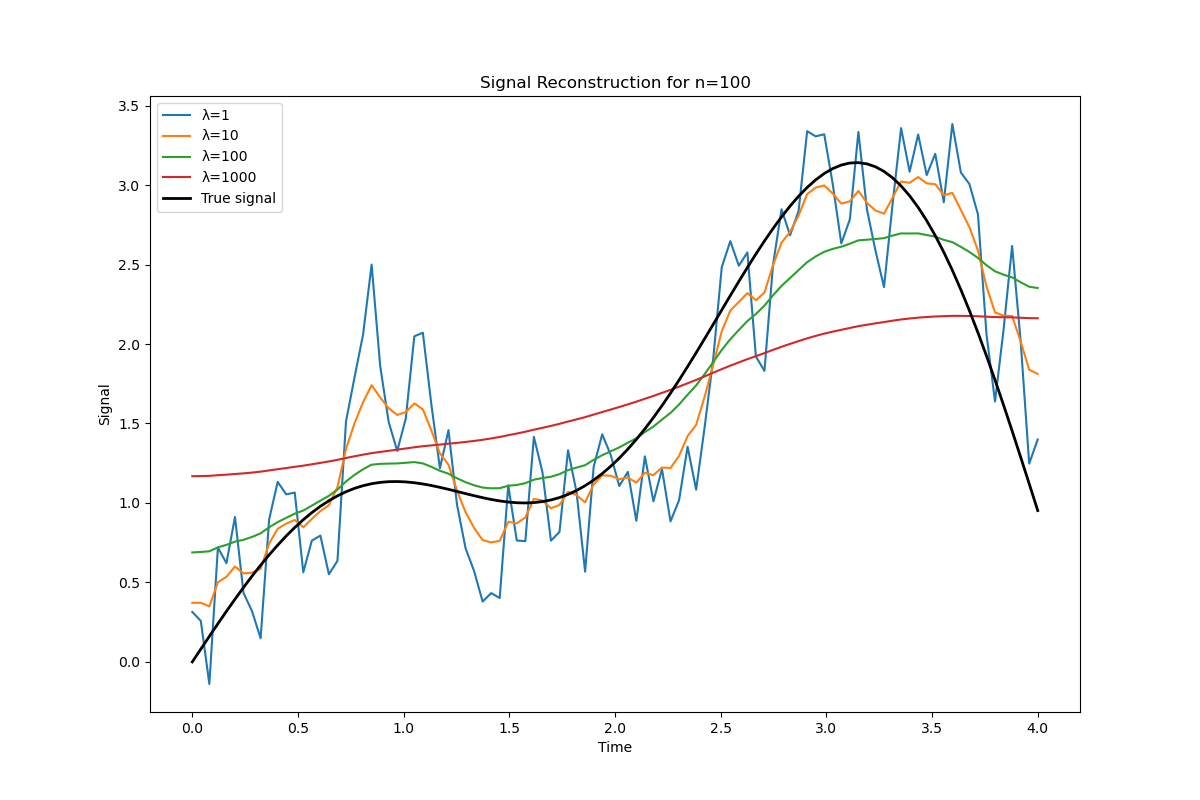
\includegraphics[height=2.0in]{signalplot_100.png}
        \caption{Signal reconstruction for $n=100$.}
        \label{fig:signal100}
    \end{subfigure}%
    ~ % This adds a little space and allows the figures to be side by side
    \begin{subfigure}[t]{0.5\textwidth}
        \centering
        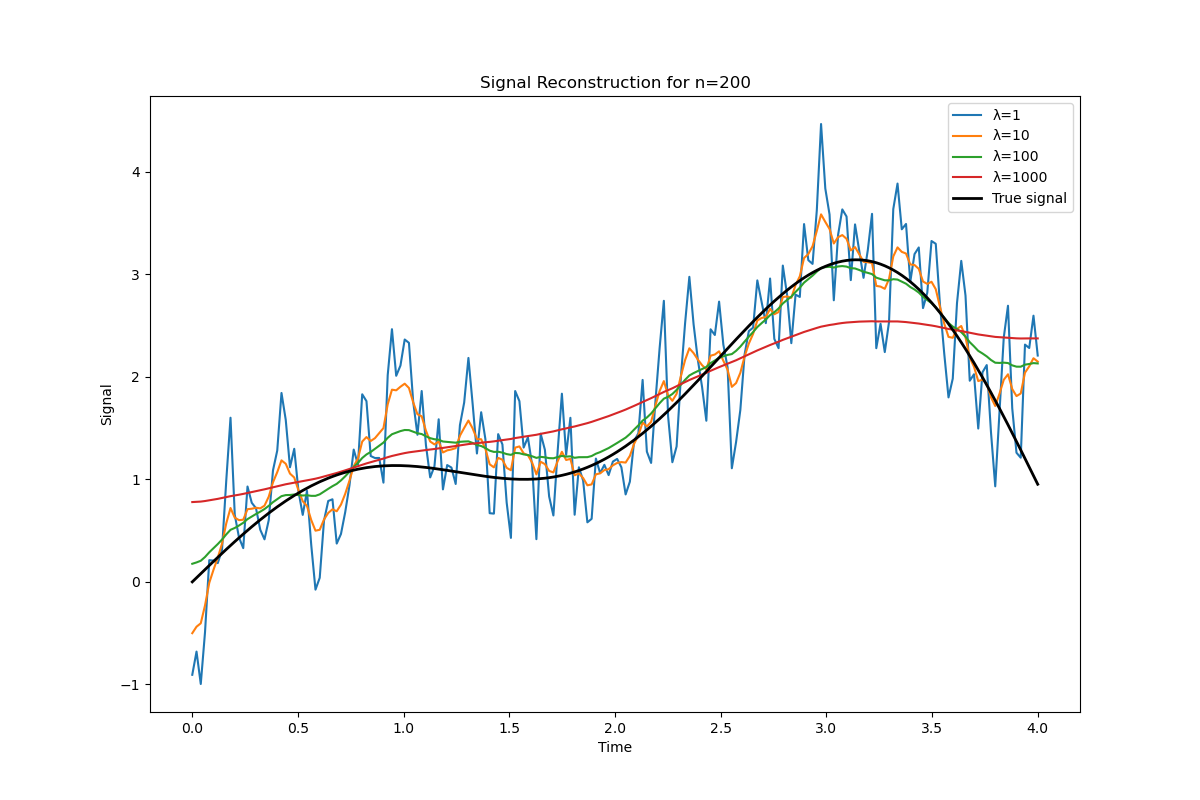
\includegraphics[height=2.0in]{signalplot_200.png}
        \caption{Signal reconstruction for $n=200$.}
        \label{fig:signal200}
    \end{subfigure}
    
    % Second row with two images
    \begin{subfigure}[t]{0.5\textwidth}
        \centering
        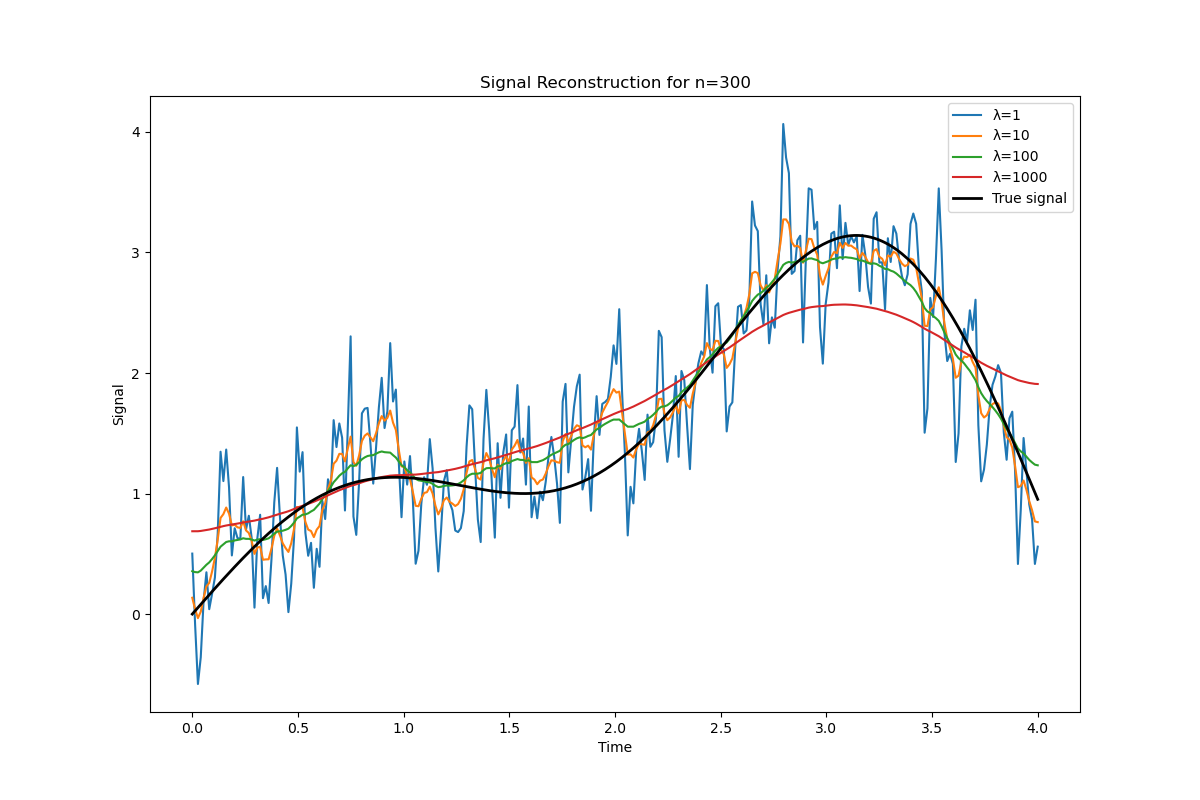
\includegraphics[height=2.0in]{signalplot_300.png}
        \caption{Signal reconstruction for $n=300$.}
        \label{fig:signal300}
    \end{subfigure}%
    ~ % This adds a little space and allows the figures to be side by side
    \begin{subfigure}[t]{0.5\textwidth}
        \centering
        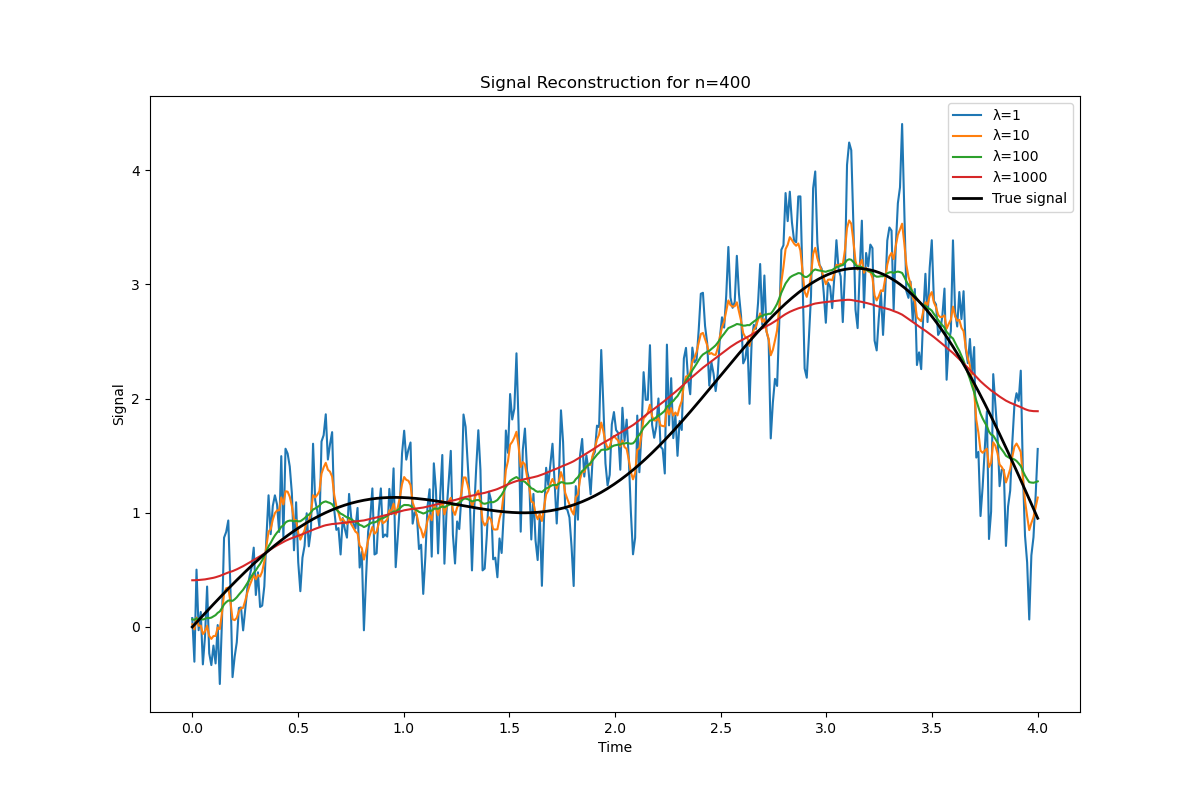
\includegraphics[height=2.0in]{signalplot_400.png}
        \caption{Signal reconstruction for $n=400$.}
        \label{fig:signal400}
    \end{subfigure}
    
    % Third row with one image centered
    \begin{subfigure}[b]{0.5\textwidth}
        \centering
        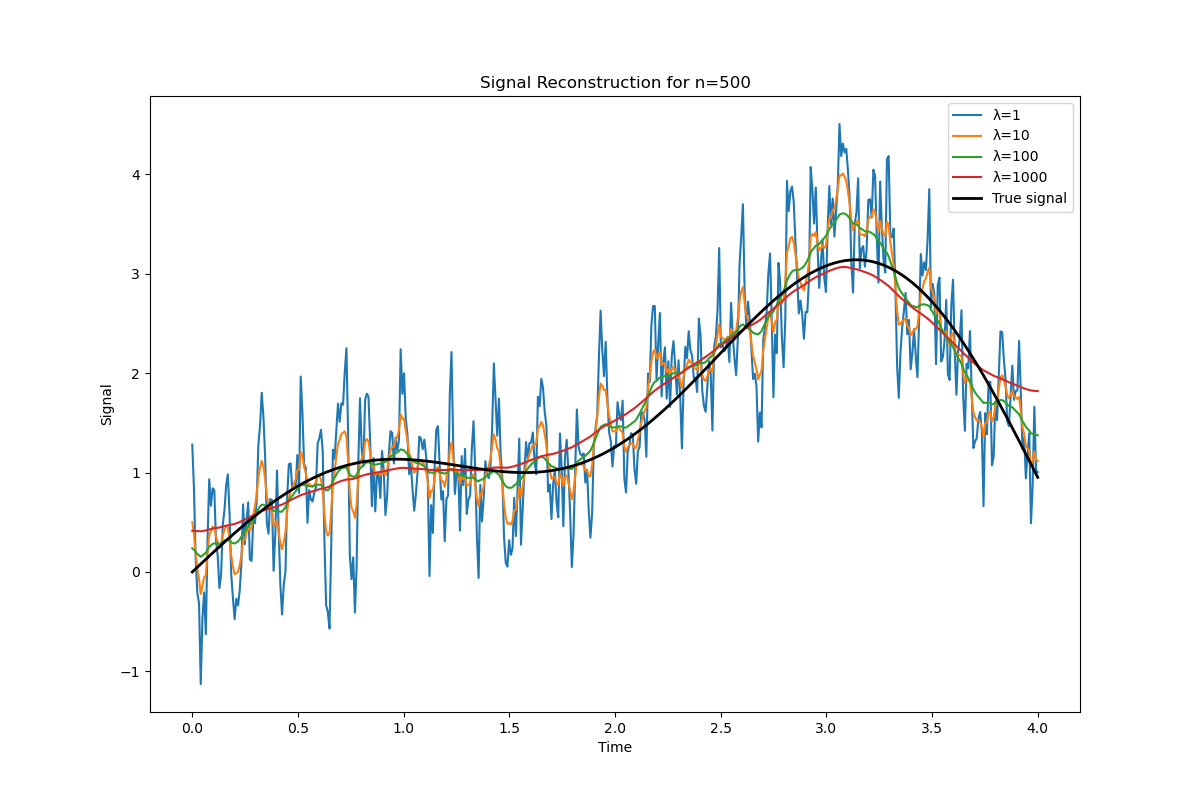
\includegraphics[height=2.0in]{signalplot_500.png}
        \caption{Signal reconstruction for $n=500$.}
        \label{fig:signal500}
    \end{subfigure}
    
    \bigskip % Adds extra space before the text for error plots
    The relative error and the condition number plots from the experiments are as follows:
    
    \begin{subfigure}[b]{.45\textwidth}
        \centering
        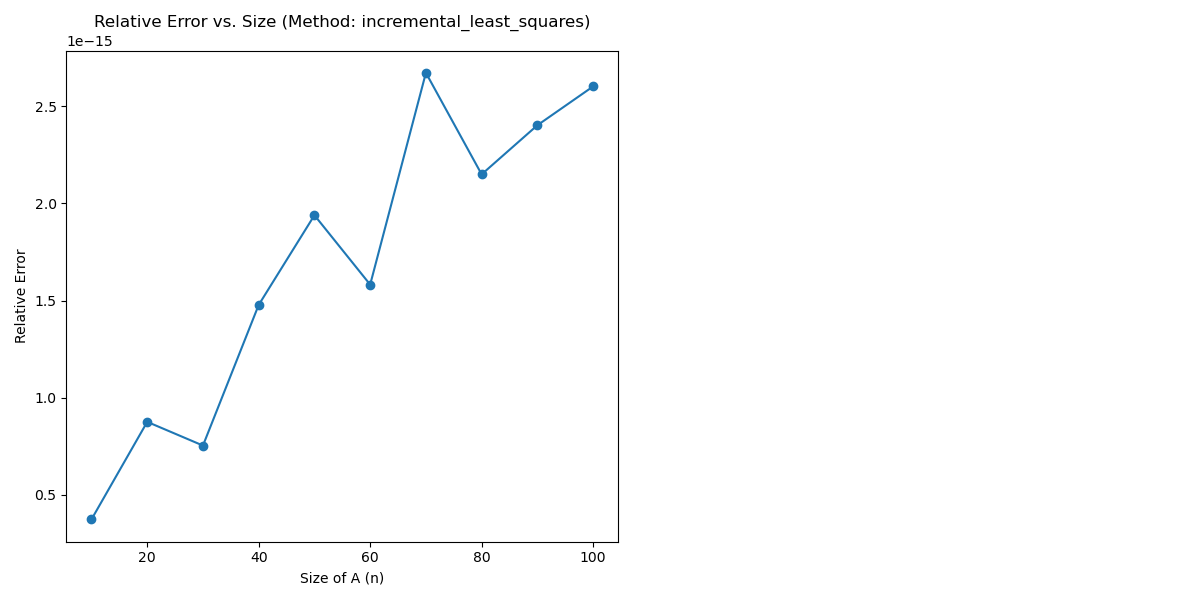
\includegraphics[width=\linewidth]{errorplot_incremental_least_squares.png}
        \caption{Relative error vs. problem size for the incremental least squares method.}
        \label{fig:error_incremental}
    \end{subfigure}
    ~ % This adds a little space between figures
    \begin{subfigure}[b]{.45\textwidth}
        \centering
        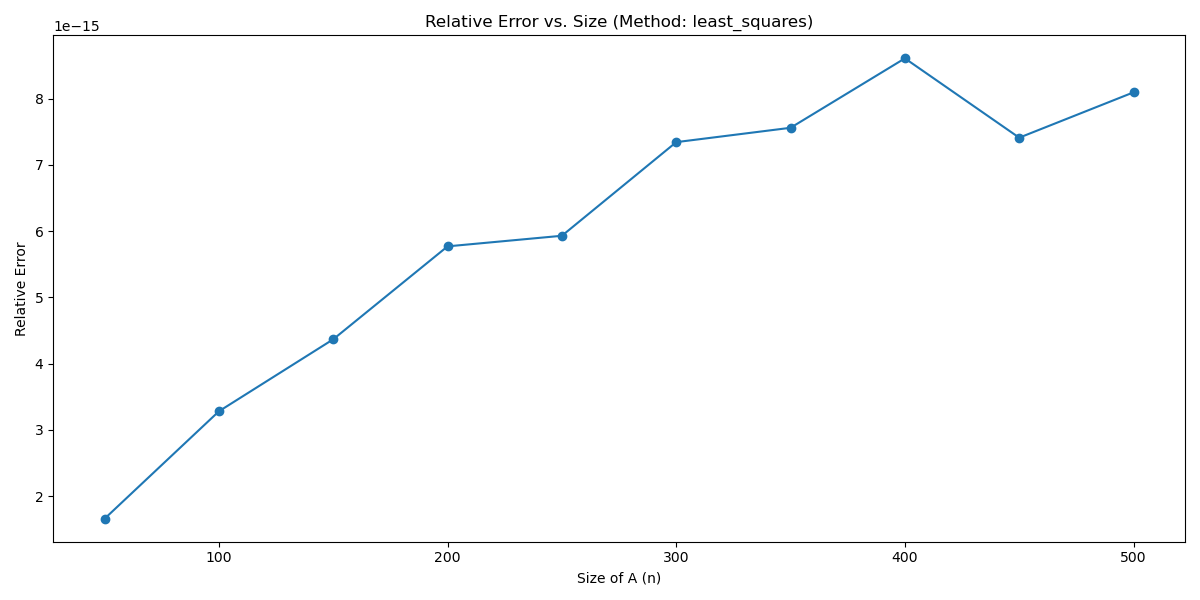
\includegraphics[width=\linewidth]{errorplot_least_squares.png}
        \caption{Relative error vs. problem size for the traditional least squares method.}
        \label{fig:error_least_squares}
    \end{subfigure}
\end{figure*}

\section{Discussion}
The results indicate the importance of choosing an appropriate $\lambda$ in regularized problems. The incremental approach, while efficient, requires careful consideration of numerical stability as the problem size grows. Comparatively, the traditional method remains robust across all tested sizes.

\section{Conclusion}
The implemented linear and regularized linear least squares methods successfully address the minimization problems, with the regularization parameter being essential for noise mitigation. These methods exhibit potential for application in real-time signal processing and other areas requiring robust statistical analysis.

\section{References}
Any papers, books, or articles referenced would be listed here.

\section{Appendices}
\subsection{Code Listings}
\begin{lstlisting}[language=Python, caption=Linear Least Squares Implementation]
# Insert your Python code for the linear least squares implementation here.
\end{lstlisting}

\begin{lstlisting}[language=Python, caption=Regularized Linear Least Squares Implementation]
# Insert your Python code for the regularized linear least squares implementation here.
\end{lstlisting}

% Include additional code listings if necessary.

\end{document}
